\documentclass[a4paper, 12pt]{report}

%%%%%%%%%%%%
% Packages %
%%%%%%%%%%%%

\usepackage[english]{babel}
\usepackage[noheader]{packages/sleek}
\usepackage{packages/sleek-title}
\usepackage{packages/sleek-theorems}
\usepackage{packages/sleek-listings}
\usepackage{xcolor}
\usepackage{graphicx}
\usepackage{hyperref}
\graphicspath{ {./images} }

\definecolor{codegreen}{rgb}{0,0.6,0}
\definecolor{codegray}{rgb}{0.5,0.5,0.5}
\definecolor{codepurple}{rgb}{0.58,0,0.82}
\definecolor{backcolour}{rgb}{0.95,0.95,0.92}

\lstdefinestyle{mystyle}{
    backgroundcolor=\color{backcolour},   
    commentstyle=\color{codegreen},
    keywordstyle=\color{magenta},
    numberstyle=\tiny\color{codegray},
    stringstyle=\color{codepurple},
    basicstyle=\ttfamily\footnotesize,
    breakatwhitespace=false,         
    breaklines=true,                 
    captionpos=b,                    
    keepspaces=true,                 
    numbers=left,                    
    numbersep=5pt,                  
    showspaces=false,                
    showstringspaces=false,
    showtabs=false,                  
    tabsize=2
}

\lstset{style=mystyle}

%%%%%%%%%%%%%%
% Title-page %
%%%%%%%%%%%%%%

\logo{./images/hu_logo.jpeg}
\institute{Habib University}
% \faculty{DSSE}
\department{CS330L Computer Architecture Lab}
\title{Lab Project Report}
\subtitle{Instructor: Maria Samad}
\author{Muhammad Hammad Maqdoom \textit{mm05534} \\ Zoha Ovais Karim zk05617 \\ Umema Zehra}
%\supervisor{Linus \textsc{Torvalds}}
%\context{Well, I was bored...}
\date{Spring 2021}

%%%%%%%%%%%%%%%%
% Bibliography %
%%%%%%%%%%%%%%%%

% \addbibresource{./resources/bib/references.bib}

%%%%%%%%%%
% Others %
%%%%%%%%%%

\lstdefinestyle{latex}{
    language=TeX,
    style=default,
    %%%%%
    commentstyle=\ForestGreen,
    keywordstyle=\TrueBlue,
    stringstyle=\VeronicaPurple,
    emphstyle=\TrueBlue,
    %%%%%
    emph={LaTeX, usepackage, textit, textbf, textsc}
}

\FrameTBStyle{latex}

\def\tbs{\textbackslash}

%%%%%%%%%%%%
% Document %
%%%%%%%%%%%%

\begin{document}
    \maketitle
    \romantableofcontents
    \chapter{Introduction}
    
    This project required us to build a 5-stage pipelined processor capable of executing a bubble sort program.
    
    \begin{enumerate}
        \item We modified the single-cycle processor to be able to run the bubble sort code on it.
        \item We then modified the said processor to make it a pipelined one (5 stages). We then tested and run each instruction separately to verify that the pipelined version can at least execute one instruction correctly in isolation.
        \item We then introduced circuitry to detect hazards (data, control, and structural) and tried to handle them in hardware i.e. by forwarding, stalling, and flushing the pipeline.

    \end{enumerate}
    
    
    \chapter{Task 1}
    \section{\texttt{Modify single-cycle processor}}
    The tasks that we attempted in lab 11 came in handy for this task. We made changes and alterations to the code in line with task 1 given to us. 
    
    We modified the single-cycle processor to be able to run the bubble sort code on it.
    We had worked on the bubble sort task in lab 4 (task 2). 
    For the instructions, we made use of the venus simulator and then used the same instructions in verilog for instruction memory. 


    \lstinputlisting[language=verilog]{./code/task1-design.v}
    Test Bench:
    \lstinputlisting[language=verilog]{./code/task1-tb.v}
    \newpage
    Result from Test Bench: \newline
    Wave Diagram \newline
    \begin{center}
        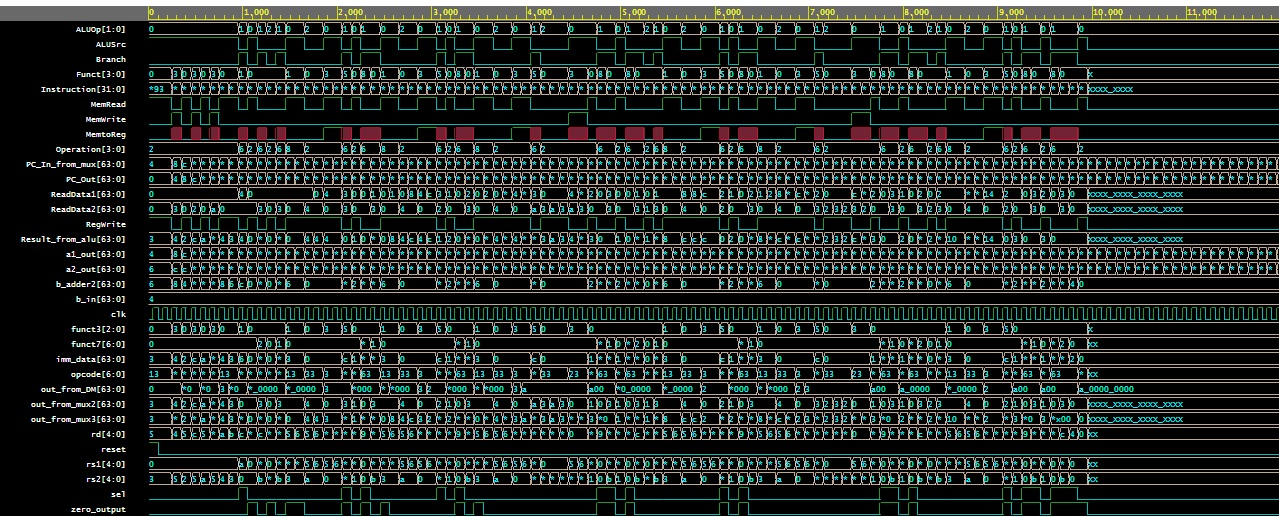
\includegraphics[width=165mm]{images/task1.jpg}
    \end{center}
   
   \chapter{Task 2}
    \section{\texttt{5 Stage Pipelining}}
    We now modified the said processor to make it a pipelined one (5 stages). We then tested and ran each instruction separately to verify that the pipelined version can at least execute one instruction correctly in isolation.

    \lstinputlisting[language=verilog]{./code/task2-design.v}
    Test Bench:
    \lstinputlisting[language=verilog]{./code/task2-tb.v}
%   \includegraphics[width=180mm]{l-11.jpg}
   
   
%   \chapter{Task 3}
%     \section{\texttt{Hazard Circuitry}}
    
%     \lstinputlisting[language=verilog]{./code/task3-design.v}
%     Test Bench:
%     \lstinputlisting[language=verilog]{./code/task3-tb.v}
%   \includegraphics[width=180mm]{l-11.jpg}
    
   \chapter{Code}
    \section{\texttt{EDA Links}}
    
    \href{https://edaplayground.com/x/NxwY}{Task 1 EDA Link}
    
    \href{https://edaplayground.com/x/G8_E}{Task 2 EDA Link}
        
    % \href{https://www.edaplayground.com/x/Dzti}{Task 3 EDA Link}


    % \lstinputlisting[language=verilog]{all.v}


\end{document}
